\scanpage{294}
\margin{\figure{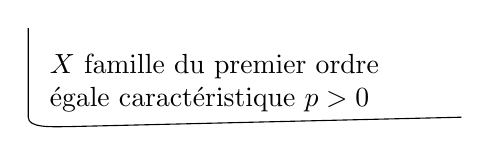
\begin{tikzpicture}\node[align=left,anchor=west] at (0.15,0.55) {$X$ famille du premier ordre\\égale caractéristique $p>0$};\draw (0,1.25)--(0,0.12)..controls (0,-0.02) and (0.3,0)..(0.5,0)--(5.5,0.12);\end{tikzpicture}}}
\diagram{\begin{tikzcd}[column sep=small]
&\uline{\operatorname{Pic}}^{\unsure{00|\infty}}_{X/\unsure{U|S}}\text{ existe}\arrow[d,Leftrightarrow]&&\\
\check V\arrow[r,"\mu"']&H^1(X_0,\unsure{\uline{\mathfrak g}_{X_0}|\uline{\mathcal T}_{X_0}})\arrow[r,"u"']&H^1(X_0,\mathcal O_{X_0})\otimes t_{B_0}\simeq&H^1(X_0,\mathcal O_{X_0})\otimes H^1(A_0,\mathcal O_{A_0})\\
&&&H^1(A_0,\uline{\mathfrak g}_{A_0})\simeq t_{A_0}\otimes H^1(A_0,\uline{\mathcal O}_{A_0})\arrow[u,"v"']
\end{tikzcd}}
\[
\operatorname{Im}u\mu\subset\operatorname{Im}v
\]
\figure{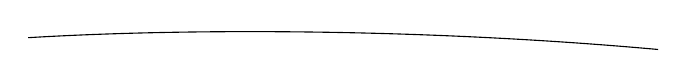
\begin{tikzpicture}\draw (0,0)..controls (2,0.12) and (5,0.12)..(8,-0.15);\end{tikzpicture}}

\diagram{\begin{tikzcd}[column sep=small,row sep=large]
\uline{\operatorname{Pic}}_{X/\unsure{U|S}}\text{ plat sur }S\text{ en }x_0\arrow[d,Rightarrow]&&V\otimes H^{\unsure{2|1}}(X_0,\uline{\mathcal O}_{X_0})\arrow[d,equal]\\
H^1(X_0,\uline{\mathcal O}_{X_0}^{*})\arrow[r,"\partial"']\arrow[dr,"\unsure{d}"']&\operatorname{Hom}(H^1(X_0,\uline{\mathfrak g}_{X_0}),H^{\unsure{2|1}}(X_0,\uline{\mathcal O}_{X_0}))\arrow[r,"\rho"']&\deleted{\operatorname{Hom}}(\check V,H^{\unsure{2|1}}(X_0,\uline{\mathcal O}_{X_0}))\\
&H^1(X_0,\uline{\Omega}^1_{X_0})\arrow[u,"c\ \text{cup}"']&
\end{tikzcd}}
\[
\rho\partial(x)=0\quad\Longleftrightarrow\quad\rho c(x)=0
\]
N.B. Cette condition est automatiquement vérifiée en les pts \inserted{\textcircled{$x_0$}} de $\uline{\operatorname{Pic}}^{\unsure{\sigma|0}}_{X_0/k}\deleted{\unsure{(X_0/k)}}$, mais il est douteux que $\uline{\operatorname{Pic}}^0_{X/k}$ soit pour autant plat sur $S$.
\margin{car $\operatorname{Pic}^0_{X/k}(k)$ est ``divisible par $p$''}
\figure{
\begin{tikzpicture}\draw (0,0)..controls (3,0.22) and (6,0.22)..(8,0.28);\end{tikzpicture}}
\mspage{293}
